\scanpage{86}
\uline{5.1.84}

J'ai vérifié que si $\mathcal X$ désigne la
surface des pos. rel. non supersingulières,
sans bord en permettant le franchissement
des positions supersingulières
par une arête ou par un sommet
(\unsure{copulations} des \uline{poids $0$}), alors que les
autres opérations qui \unsure{s'y interprètent}
par le côté, \unsure{donnent|donne} les spéc. et gén.
ordinaires (i.e. des poids $\pm1$) --- alors
\[
\pi_1(\mathcal X,D)\longrightarrow\mathbb D_{2n}
\quad\text{(en fait : }\operatorname{Aut}\operatorname{Pol}(\unsure{D_{\mathrm{am}}})\text{)}
\]
était surjectif --- son image contient,
pour une arête ou un \deleted{\unsure{g}} sommet
donné en $D$, la symétrie p.r.
cette arête ou sommet, par le lacet
corresp. et à une ``\uline{demi torsion}'' de $D$
autour du \deleted{\unsure{cet}} sommet, ou cette
arête. Ceci ne prouve pas que
\[
\pi_1(\widetilde{\mathcal X},D)\longrightarrow
\operatorname{Aut}\operatorname{Pol}(D)\simeq\mathbb D_{2n}
\]
soit surjectif, si $\widetilde{\mathcal X}$ désigne le \unsure{découpage}
de $\mathcal X$ le long des lieux supercritiques
--- i.e. en exclut le franchissement des
positions supersingulières. Le raisonnement
montre seulement que l'image contient
les symétries p.r. à \deleted{\unsure{l'autre}} \uline{arête} (mais pas
néc. p.r. à un sommet). \deleted{\unsure{Celles symétries}}
engendrent ds $\mathbb D_{2n}$ un \deleted{sous} groupe
d'indice $2$, à savoir celui formé par les
\deleted{rotations} les élts du sous-groupe
de rotations $\mathbb D_n^+$ (d'ordre \uline{$n$}, non $2n$),
et les réflexions en question. [NB. C'est
un des trois sous-groupes d'indice deux,
les deux autres étant le groupe engendré
par les \deleted{\unsure{sym}} réflexions qui \unsure{inversent} \deleted{\unsure{les}}
un sommet, et le sous-groupe $\mathbb D_{2n}^+$
des rotations.] L'image de $\pi_1(\widetilde{\mathcal X})$ ds $\mathbb D_{2n}$
est donc d'indice $1$ ou $2$.

Faisant un \deleted{\unsure{demi tour}} \inserted{demi} tour \deleted{complet}
autour d'une position supersingulière,
\inserted{par le franchissement, \unsure{tout des effets sur}}
\deleted{\unsure{dans l'opération de rotation par}}
\inserted{(sur $\operatorname{Pol}(D)$) qui \unsure{se fait|définit} par une rotation}
\deleted{\unsure{(sur) un cercle par $\pi/2$}, \unsure{fait une} \uline{\unsure{demi}}}
\deleted{\unsure{tour}} \inserted{d'un facteur} \unsure{$n+1$} --- si $n$ est \deleted{pair}
impair, cela montre que l'effet sur
l'ensemble \deleted{des \unsure{p.}} \inserted{$\varepsilon_a(D)$} des \deleted{\unsure{poly}}gones
circonscrits (et aussi sur les deux autres
ens. à deux éléments $\varepsilon_s(D)$, $\uline{\omega}(D)$)
est le $=$. \deleted{\unsure{que}} Donc pour voir si $\forall$
lacet en $D_0$ \deleted{fixé}, donne \deleted{fixe}

\margin{\unsure{J'ai été assez négligent}
\unsure{dans l'explicitation de la règle}
\unsure{de recollement des flèches} de transition
exceptionnelles.}
\margin{\unsure{reste trop conjectural}; \unsure{en fait} $\deleted{\unsure{+}}1$ \unsure{au lieu} \unsure{de}
\unsure{l'angle} \unsure{ci-dessus}. \unsure{Mais c'est l'angle}.}
\figure{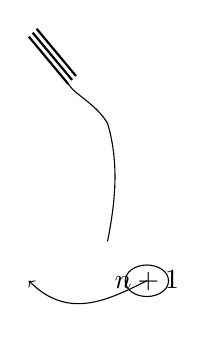
\begin{tikzpicture}[x=.5cm,y=.5cm]
\draw (0,0)..controls(.2,1)and(.3,2)..(0,3);
\draw (0,3)..controls(-.3,3.5)and(-.8,3.7)..(-1,4);
\draw[line width=.8pt](-1,4)--(-2,5.2) (-.9,4.1)--(-1.9,5.3) (-.8,4.2)--(-1.8,5.4);
\draw[->](1,-1)..controls(0,-1.5)and(-1,-2)..(-2,-1);
\draw (1,-1) ellipse(.55 and .4);
\node at (1,-1){$n+1$};
\end{tikzpicture}}
\margin{85}
